
\section{Reproducibility Setup}
\label{sec:reproducibility_setup}

A key goal of the RollupX benchmark suite is to make each experiment repeatable under the same configuration and environment assumptions. The benchmark matrix is executed using the \texttt{run\_matrix.sh} wrapper script, which reads the experiment definitions from \path{experiments.toml} and runs the selected benchmark configurations sequentially.

Before each run, the wrapper resets the local environment to reduce state leakage between experiments. This includes tearing down the Docker stack, clearing internal SQLite databases, and removing stale service state that could otherwise affect nonce handling, batch identifiers, or metric outputs. After the reset step, the local Layer-1 node and RollupX services are started again, the required contracts are deployed or reused, and the selected workload is executed.

\begin{figure}[!htbp]
    \centering
    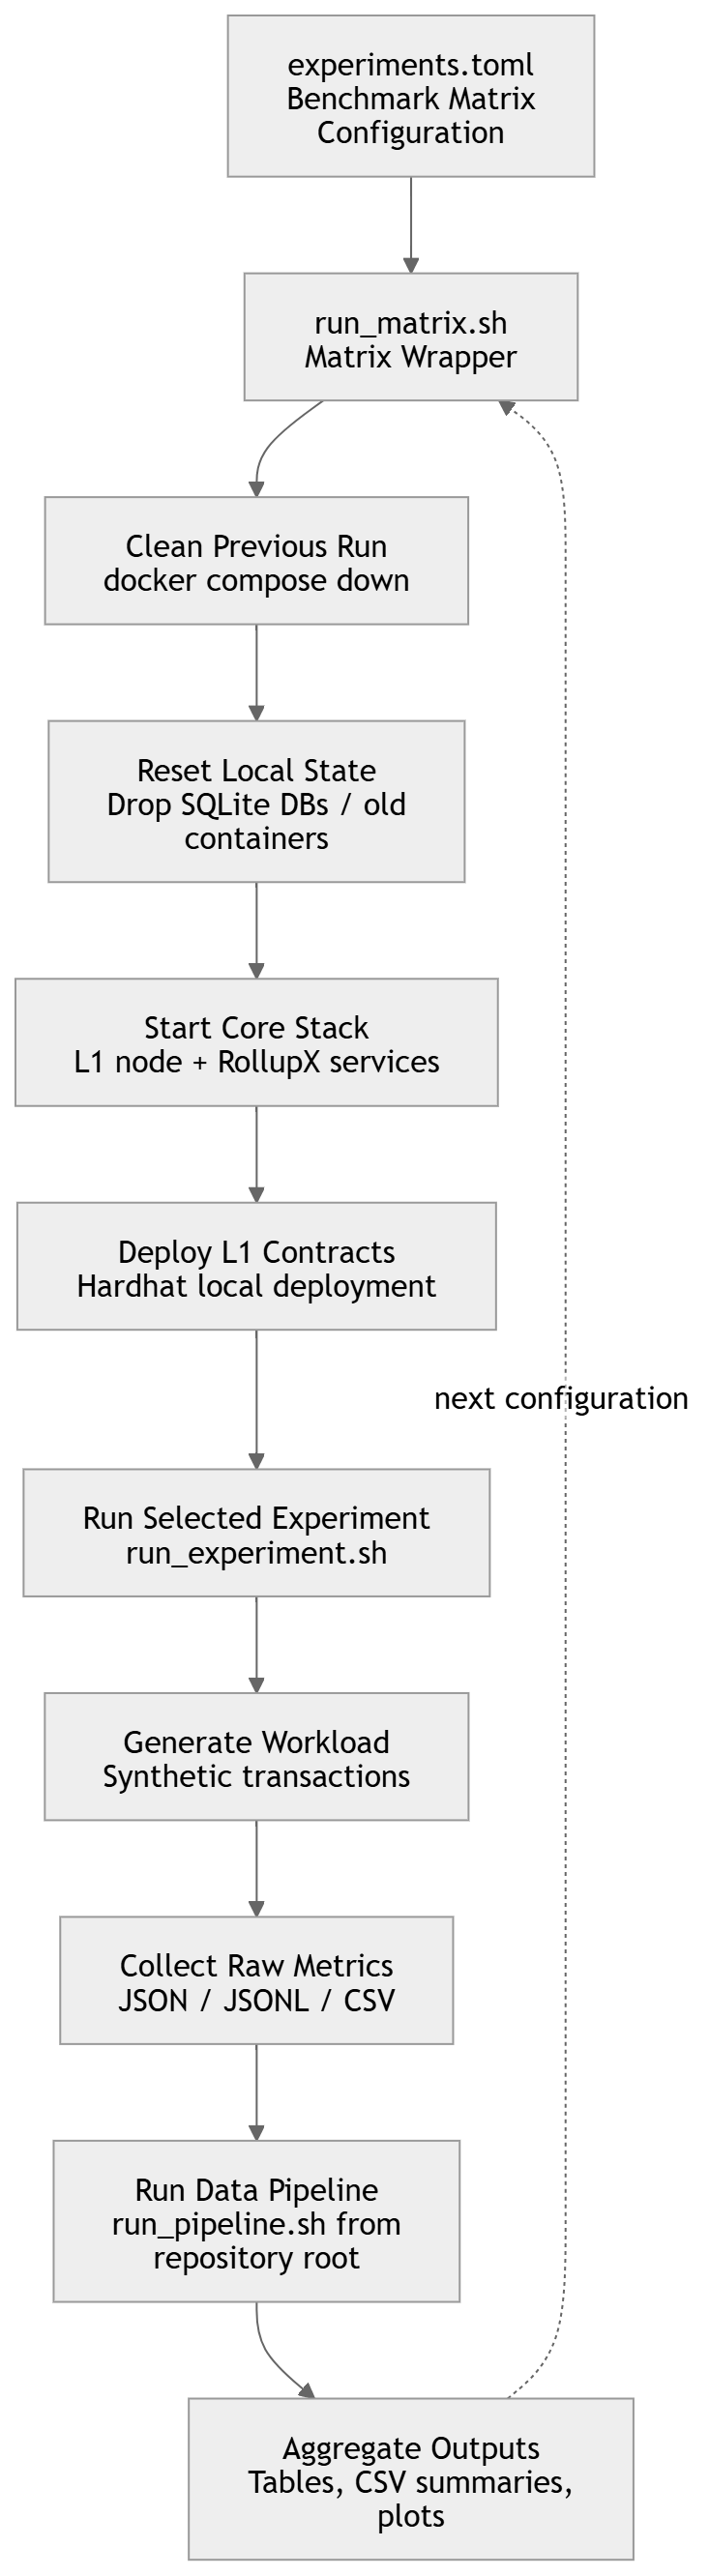
\includegraphics[
        width=0.42\textwidth,
        keepaspectratio
    ]{figures/chapter5/reproducibility_workflow.png}
    \caption{RollupX benchmark reproducibility workflow.}
    \label{fig:reproducibility_workflow}
\end{figure}

Figure~\ref{fig:reproducibility_workflow} shows the reproducibility workflow followed by the benchmark suite. The process begins with the experiment matrix configuration, followed by environment reset, stack initialization, benchmark execution, metrics export, and result aggregation. The same workflow is repeated for each configuration in the matrix, allowing benchmark results to be compared under controlled conditions.

The main commands used to reproduce the benchmark workflow are summarized in Table~\ref{tab:reproducibility_commands}.

\begin{table}[!htbp]
\centering
\caption{Reproducibility Commands}
\label{tab:reproducibility_commands}
\small
\setlength{\tabcolsep}{4pt}
\renewcommand{\arraystretch}{1.15}
\begin{tabularx}{\textwidth}{@{}>{\raggedright\arraybackslash}p{0.43\textwidth}X@{}}
\toprule
\textbf{Command / script} & \textbf{Purpose} \\
\midrule

\texttt{docker compose --profile core up -d}
& Starts the foundational local benchmark stack, including the Layer-1 node and core RollupX services. \\

\addlinespace

\texttt{npx hardhat run scripts/deploy-local.ts --network localhost}
& Deploys the Layer-1 settlement contracts manually when Docker-based automation is not used. \\

\addlinespace

\texttt{benchmark-suite/scripts/run\_matrix.sh}
& Executes the full benchmark matrix by iterating through the configurations defined in \path{experiments.toml}. \\

\addlinespace

\texttt{benchmark-suite/scripts/run\_experiment.sh}
& Executes a selected benchmark scenario or configuration sweep. \\

\addlinespace

\texttt{bash run\_pipeline.sh}
& Runs the Python data-tools aggregation pipeline from the repository root and generates summarized result outputs. \\

\bottomrule
\end{tabularx}
\normalsize
\end{table}

It is important to execute \texttt{run\_pipeline.sh} from the repository root directory rather than from inside \path{benchmark-suite/}. The aggregation scripts depend on relative paths to the \path{data-tools/} directory and benchmark output folders. Running the pipeline from the wrong directory can cause missing-file errors or incomplete aggregation outputs.

Overall, this setup improves reproducibility by making each benchmark run configuration-driven, isolated, and repeatable. The use of \path{experiments.toml}, Docker-based orchestration, environment cleanup, and a fixed aggregation pipeline allows the same benchmark matrix to be rerun after implementation changes or parameter adjustments.

